\documentclass[12pt]{article}

% Packages to include in document.
\usepackage[margin=.75in]{geometry}
\usepackage{amsmath}
\usepackage{amssymb}
\usepackage{mathtools}
\usepackage{setspace}
\usepackage{float}
\usepackage[hidelinks]{hyperref}
\usepackage[noabbrev,capitalize,nameinlink]{cleveref}
\usepackage[compact]{titlesec}
\usepackage{amsthm}
\usepackage{caption}

% Reduce spacing around section labels and headers.
\titlespacing{\section}{0pt}{*0}{*0}
\titlespacing{\subsection}{0pt}{*0}{*0}
\setlength{\headheight}{15pt}
\setlength{\headsep}{12pt}

% amsthm definition style, numbering follows sections.
\newtheorem{theorem}{Theorem}%[section]

% Commonly used commands.
\newcommand{\set}[1]{\ensuremath{\left\{#1\right\}}}
\newcommand{\E}{\ensuremath{\mathbb{E}}}
\newcommand{\given}{\,|\,}

\title{
  Consistently Correct \\
  \large Leveraging eventual consistency to attain eventual correctness \\ in a multi-writer \& multi-replica environment
}
\author{Andrew Wang}
\date{2024-11-29}
\doublespacing

\begin{document}
\maketitle
The following paper is transposed from a presentation given at Amazon. It's motivated by the need to coalesce numerical data from multiple regions into a single source of truth.
\tableofcontents

\section{Definitions}

Consider a system of \(m\) independent writers sending data to \(n\) data store replicas, where any writer can send data to any replica. An example is shown in \cref{scenario_img}. In \cref{writers} and \cref{replicas}, we define properties of the writers and replicas, respectively. In \cref{objective}, we set the goals that our system must achieve.

\begin{figure}[htbp]
	\centering
	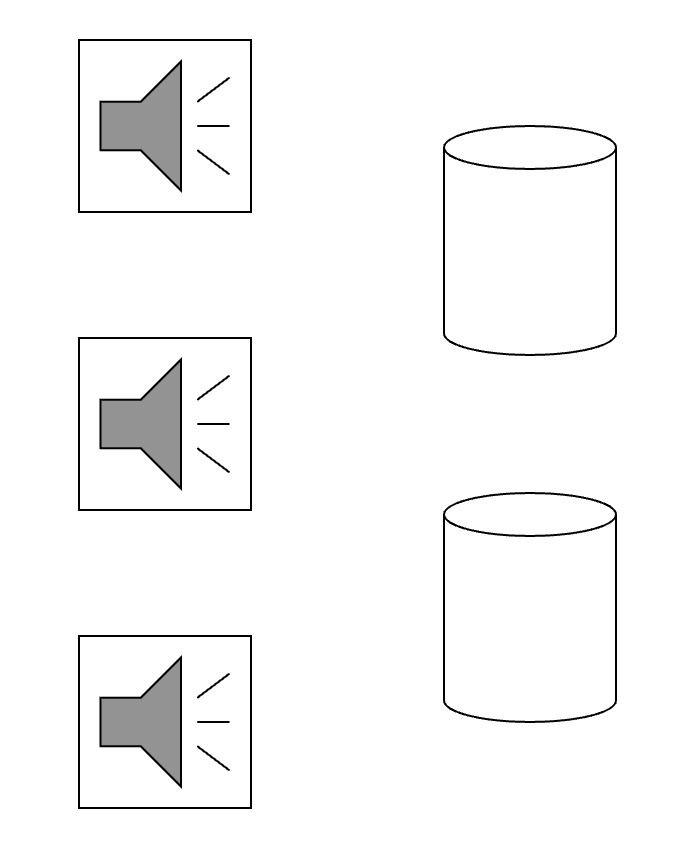
\includegraphics[width=.45\textwidth]{objective.png}
	\caption{\(m=3\) writers and \(n=2\) replicas.}
	\label{scenario_img}
\end{figure}

\subsection{Writers} \label{writers}

The writers satisfy the following conditions:
\begin{description}
	\item[Independence] Writers are stateless and cannot communicate with one another.

	\item[Fallibility] A writer can emit a wrong value with fixed probability \(\alpha\).

	\item[Ordered] The possible data values constitute a totally/linearly ordered set.
\end{description}

\subsection{Replicas} \label{replicas}

The replicas are based on \href{https://aws.amazon.com/dynamodb/global-tables/}{Amazon DynamoDB global tables} and satisfy the following conditions:
\begin{description}
	\item[Convergence] Data store replicas follow a ``last write wins'' eventual consistency model.
	
	\item[Conditional] The replicas support conditional updates based on the total order.
	
	\item[Ordered] The greater a value is with respect to the total ordering, the more ``correct'' it is. 
\end{description}
Conditional updates are based on the \href{https://docs.aws.amazon.com/amazondynamodb/latest/APIReference/API_UpdateItem.html}{DynamoDB UpdateItem action}. The request value is compared against the replica's currently stored value, and a user-defined predicate determines whether or not to overwrite the stored value.

\subsection{Objective} \label{objective}

We seek a connection topology and algorithm that connects writers to data store replicas in a way that satisfies all 4 objectives below: 
\begin{enumerate}
	\item \textbf{Convergence:} Assuming at least 1 correct writer, guarantee that all replicas converge to the correct answer:
	\begin{enumerate}
		\item If the system is operating ideally and no messages are lost.
		
		\item Irrespective of event ordering, e.g. write requests, database replications.
	\end{enumerate}
	
	\item \textbf{Fault Tolerance:} Automatic fault tolerance against any single point of failure. No intervention should need to take place for the system to continue operation.
	
	\item \textbf{Minimalism:} Fulfills (1) and (2) with the fewest number of connections.
	
	\item \textbf{Probabilistic Guarantees:} Admits low expected error rates even under faulty operating conditions, i.e. lost messages.
\end{enumerate}

\section{Solution Topologies}

We review 2 solutions that do \emph{not} work in \cref{1_1} and \cref{act_pass}, before presenting a working solution in \cref{act_act}.

\subsection{One to One} \label{1_1}

When \(m \leq n\), we may injectively map writers to replicas. Each writer updates its corresponding replica with the data value it sends. This setup fails to converge but is fault tolerant.

\begin{figure}[htbp]
	\centering
	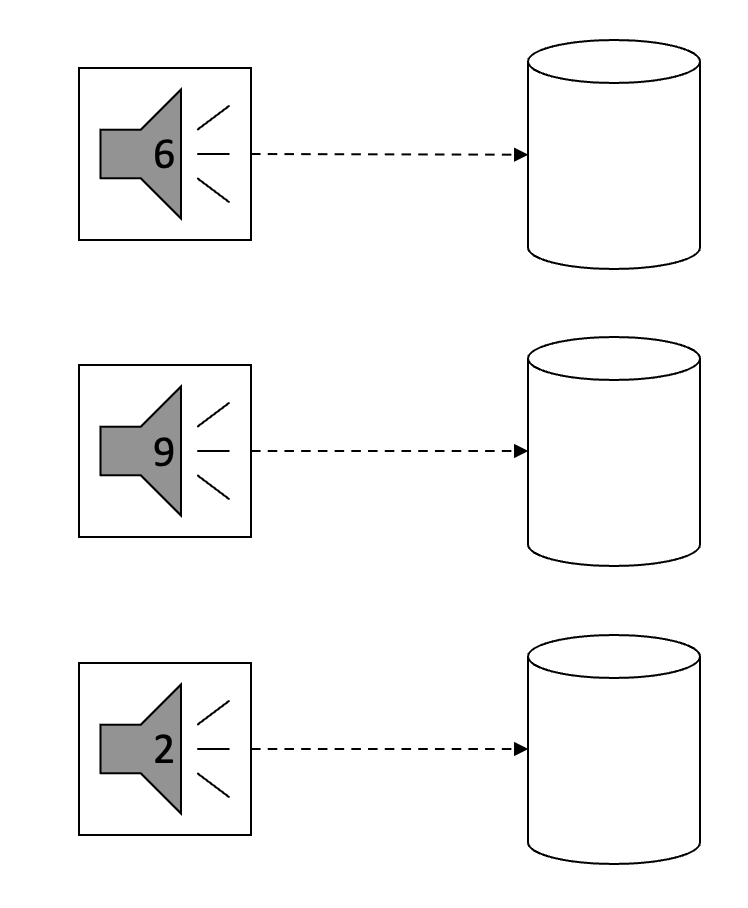
\includegraphics[width=.45\textwidth]{one_one.png}
	\caption{\(1 : 1\) Topology -- the correct value is the greatest, i.e. 9.}
	\label{one_one_img}
\end{figure}

\begin{enumerate}
	\item \textbf{Convergence:} It's evident that the \(1 : 1\) topology fails to guarantee convergence. In \cref{one_one_img}, whichever writer is the last to send its value will cause all replicas to converge to its value.
	
	\item \textbf{Fault Tolerance:} The system has no single point of failure if \(m, n > 1\). Any writer, connection, or replica can be lost without affecting the system's ability to operate as a whole.
\end{enumerate}

\subsection{Active Passive} \label{act_pass}

As shown in \cref{act_pass_img}, an active-passive topology forms an \(S_m\) star graph wherein all writers send data to a single replica. Crucially, each writer enacts a conditional update such that the active replica only updates its stored value if the request value is strictly greater than the stored value. Here, ``greater'' is defined with respect to the linear order.

\begin{figure}[htbp]
	\centering
	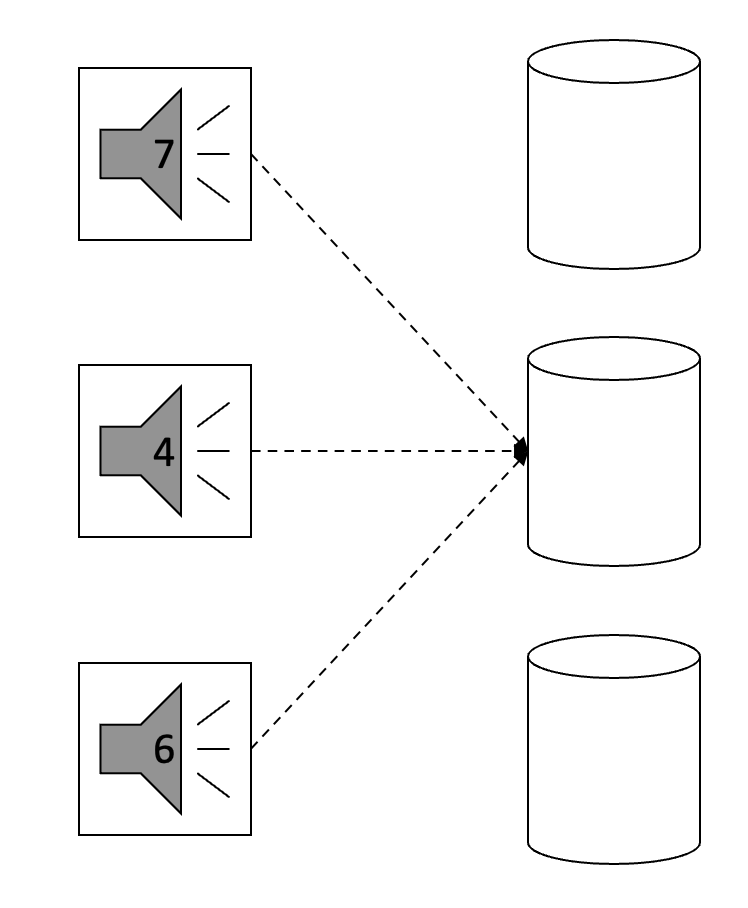
\includegraphics[width=.45\textwidth]{act_pass.png}
	\caption{Active Passive Topology -- forming an \(S_3\) star. This system converges to 7.}
	\label{act_pass_img}
\end{figure}

The ``last updated replica'' (LUR) is the last data store replica to receive an update that changes its internal value. This concept will be important later in \cref{act_act}. In the active-passive setup, it's clear that the LUR is always the active replica. This setup converges but is not fault tolerant.
\begin{enumerate}
	\item \textbf{Convergence:} The replicas converge to the correct value, agnostic of the ordering of events. See \cref{act_pass_converge} for proof.
	
	\item \textbf{Fault Tolerance:} Any fault in the active replica will bring down the entire system. In a real-world system, this would require intervention to promote one of the passive replicas to active.
\end{enumerate}

\begin{theorem}[Active Passive Convergence] \label{act_pass_converge}
	Suppose that writers \(w_1, \dotsc, w_m\) update a single active replica. This system converges if any value is correct.
	\begin{proof}
		Assume without loss of generality that \(w_1, \dotsc, w_m\) is the ordering of write events, and let \(x_1, \dotsc, x_m\) be the value of the replica after every event. For every \(1 \leq i < m\), we update \(x_{i + 1} \gets w_{i + 1}\) if and only if \(w_{i + 1} > x_i\). This means that \(x_i \gets \max(w_1, \dotsc, w_i)\) and \(x_1 \leq \dotsm \leq x_m\) is an increasing sequence. Since \(x_m\) is the largest writer value, it's correct by definition. Finally, the LUR is always the active replica, so the system converges.
	\end{proof}
\end{theorem}

\subsection{Active Active} \label{act_act}

As shown in \cref{act_act_img}, an active-active topology forms a \(K_{m, n}\) complete bipartite graph wherein every writer sends data to every replica. Like the active-passive topology, we use conditional updates predicated on updating when the request value is greater than the stored value. In this case, the LUR might change after every write event.

\begin{figure}[htbp]
	\centering
	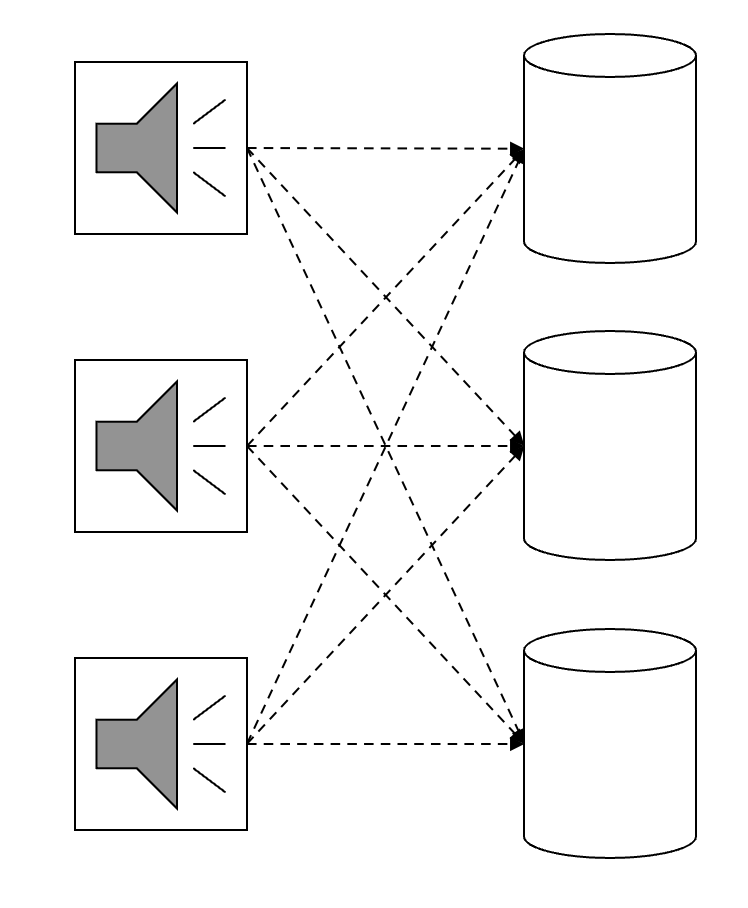
\includegraphics[width=.45\textwidth]{act_act.png}
	\caption{Active Active Topology -- forming a \(K_{3, 3}\) complete bipartite graph.}
	\label{act_act_img}
\end{figure}

We claim the following.
\begin{enumerate}
	\item \textbf{Convergence:} The replicas converge to the correct value, agnostic of the ordering of events. See \cref{act_act_converge} for proof.
	
	\item \textbf{Fault Tolerance:} No single point of failure exists when \(m, n > 1\). Loss of a writer converts the system to a \(K_{m - 1, n}\) topology. Loss of a replica converts the system to a \(K_{m, n - 1}\) topology.
	
	\item \textbf{Minimalism:} The active-active topology attains convergence and fault tolerance with the fewest number of connections. See \cref{act_act_minimal} for proof.
\end{enumerate}

\begin{theorem}[Active Active Convergence] \label{act_act_converge}
	Suppose that writers \(w_1, \dotsc, w_m\) send data to replicas \(r_1, \dotsc, r_n\). Every writer \(w_i\), \(1 \leq i \leq m\) sends its value to every data store replica \(r_j\), \(1 \leq j \leq n\). This system converges if any value is correct.
	\begin{proof}
		The base case topology of \(K_{m, 1}\) is equivalent to an active-passive \(S_m\) topology, so this is known to converge due to \cref{act_pass_converge}. Assume by way of induction that a \(K_{m, n}\) topology converges. We need to show that a \(K_{m, n + 1}\) topology converges. Define the set of replicas \(\Omega \coloneqq \set{r_1, \dotsc, r_n}\). An example is shown in \cref{induct_img}.
		
		If \(\Omega\) contains the LUR, it replicates the correct answer to \(r_{n + 1}\) by the inductive hypothesis, and we are finished. Assume by contradiction that \(r_{n + 1}\) is the LUR and that it replicates an incorrect value to \(\Omega\). This means that the last writer to update \(r_{n + 1}\) was wrong, which is a contradiction when a correct writer exists.

		Note that the value the system converges to is completely determined by the LUR due to the ``last write wins'' eventual consistency model. Different intermediary updates do not affect the final outcome when the value of the LUR is known. Since the LUR is always correct (whether in \(\Omega\) or \(r_{n + 1}\)), the active-active system converges as a whole.
	\end{proof}
\end{theorem}

\begin{figure}[htbp]
	\centering
	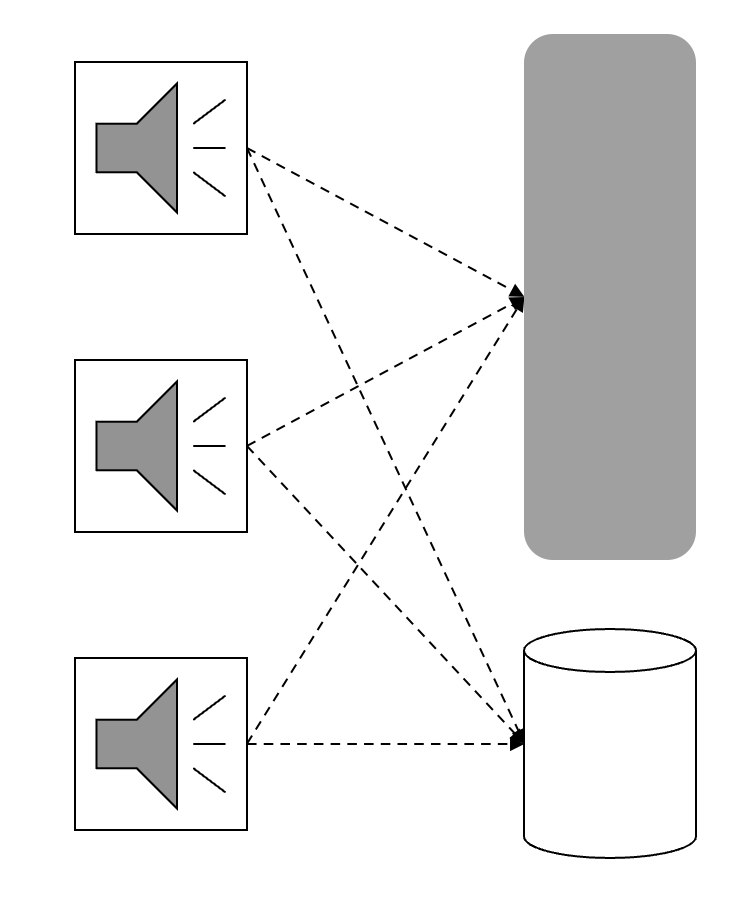
\includegraphics[width=.45\textwidth]{induct.png}
	\caption{Replicas \(1, \dotsc, n\) form a black box \(\Omega\).}
	\label{induct_img}
\end{figure}

\begin{theorem}[Active Active Minimalism] \label{act_act_minimal}
	The \(K_{m, n}\) active-active topology achieves both convergence and fault tolerance with the fewest number of connections.
	\begin{proof}
		It suffices to show that the loss of any single connection permits a sequence of write events that causes the system to converge to a wrong value. Refer to \cref{minimal_img} for an example. Suppose that writer \(w\) cannot send data to replica \(r\). If \(w\) contains the sole correct value, then \(r\) converges to the second most correct value. Furthermore, if \(r\) is the LUR, then the system fails to converge to the correct value emitted by \(w\).
	\end{proof}
\end{theorem}

\begin{figure}[htbp]
	\centering
	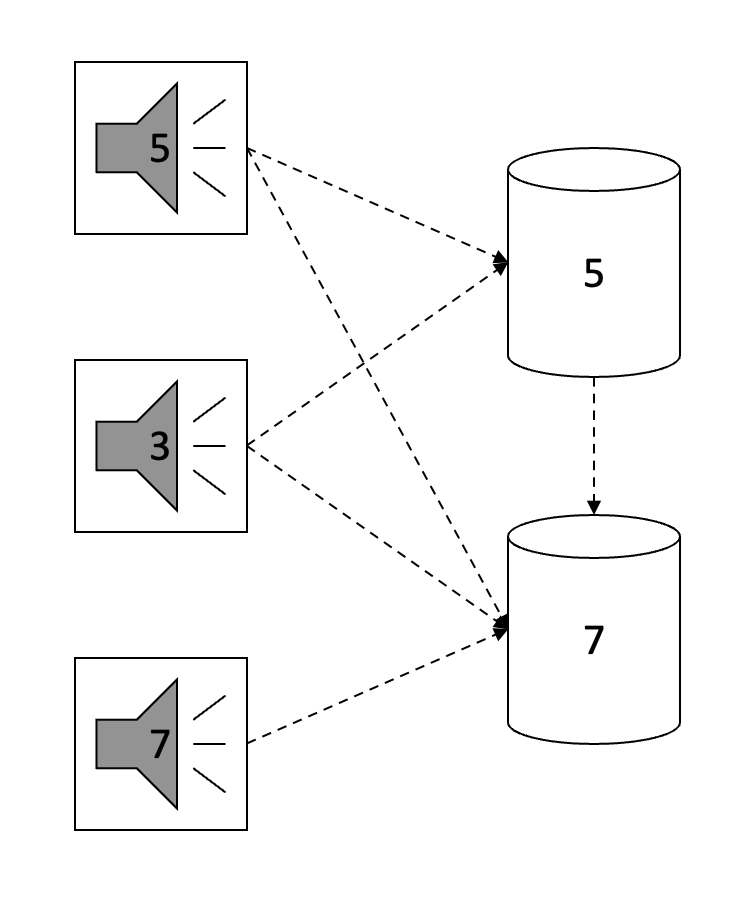
\includegraphics[width=.45\textwidth]{minimal.png}
	\caption{LUR replica with missing connection converges to 5 and updates the other replica.}
	\label{minimal_img}
\end{figure}

\section{Error Probability}

Recall that each writer has a fixed probability \(\alpha\) of emitting an incorrect value. In \cref{ideal_cond}, we show a simple example of error probability analysis when all components are available. In \cref{faulty_cond}, we compare convergence probabilities for the 3 solutions discussed when certain components are unavailable.

\subsection{Ideal Conditions} \label{ideal_cond}

As we saw earlier, if no writer, replica, or connection is unavailable, then the active-passive or active-active systems converge correctly whenever a correct writer is present. That is, the system can only converge incorrectly if \emph{every} writer emits an incorrect value. This occurs with the following probability \(P(\text{error}) = P(\text{all writers are wrong}) = \alpha^m\) for \(m\) independent writers.

For example, consider an \(S_3\) or \(K_{3, n}\) system with \(\alpha \coloneqq 0.01\). Suppose that this system propagates one value every minute. Then the number of errors that occur in a calendar year is a binomial distribution \(X\) with 525,600 trials (minutes per year) and
\begin{equation}
	\E(X) = 525600 \cdot \alpha^3 \approx 0.53
\end{equation}
The system is expected to converge to a wrong value approximately once every 2 years.

\subsection{Faulty Conditions} \label{faulty_cond}

As motivation, we derive the expression for the expected error rate of an active-active system when a single connection between writer \(w\) and replica \(r\) is lost. If any non-\(w\) writer contains the correct value, the system converges. So then,
\begin{align}
\begin{split}
	P(\text{error}) &= P(\text{error} \given \text{all writers are wrong}) + P(\text{error} \given w \text{ is the only correct writer}) \\
	&= \alpha^m +  P(r \text{ is the LUR}) \cdot P(\text{Non-}w \text{ writers are wrong}) \cdot P(w \text{ is correct}) \\
	&= \alpha^m + \frac{m - 1}{mn - 1} \cdot \alpha^{m - 1} (1 - \alpha)
\end{split}
\end{align}
Note that in \cref{comparison_tab}, a \(\star\) denotes that the expression is valid if the unavailable replica or connection is chosen from a uniform distribution amongst the available ones.

\begin{table}[htbp]
	\centering
	\doublespacing
	\caption{Topology Comparison and Expected Error Rates}
	\begin{tabular}{|c|c|c|c|}
		\hline
		& One to One & Active Passive & Active Active \\ \hline
		Convergence & \(\times\) & \checkmark & \checkmark \\ \hline
		Fault Tolerance & \checkmark & \(\times\) & \checkmark \\ \hline
		Number of Connections & \(m \leq n\) & \(m\) & \(m \cdot n\) \\ \hline
		\(\E(\text{error} \given \text{ideal conditions})\) & \(\alpha\) & \(\alpha^m\) & \(\alpha^m\) \\ \hline
		\(\E(\text{error} \given \text{dropped writer})\) & \(\alpha\) & \(\alpha^{m - 1}\) & \(\alpha^{m - 1}\) \\ \hline
		\(\E(\text{error} \given \text{dropped replica})\) & \(\alpha\) & \(\star \quad \frac{m - 1}{m} \cdot \alpha^{m - 1} + \frac{1}{m} \) & \(\alpha^m\) \\ \hline
		\(\E(\text{error} \given \text{dropped connection})\) & \(\alpha\) & \(\alpha^{m - 1}\) & \(\star \quad \alpha^m + \frac{m - 1}{mn - 1} \cdot \alpha^{m - 1} (1 - \alpha)\) \\
		\hline
	\end{tabular}
	\label{comparison_tab}
\end{table}

\end{document}